\chptr{Dinamica}
\marginpar{\minitoc}

\section{Leggi della dinamica}

Nella descrizione introduttiva del moto, non è stata analizzata alcuna causa del
fenomeno.

\subsection{La prima legge}

\vspace{8pt}
\begin{tcolorbox}[colback = red!30, colframe = red!30!black, title = {Prima legge della dinamica (legge di inerzia)}]
    Un corpo permane nel suo stato di \textit{quiete} o moto rettilineo uniforme
    finché non intervenga un \textit{agente esterno}.
\end{tcolorbox}
\vspace{5pt}

In altre parole, se nulla ``rompe le scatole'' al corpo, esso permanerà nel suo
stato di moto, naturalmente.

\vspace{8pt}
\begin{tcolorbox}[colback = yellow!30, colframe = yellow!30!black, title = {Sistema inerziale}]
    Sistema nel quale vale la prima legge della dinamica.
\end{tcolorbox}
\vspace{5pt}

\subsection{La seconda legge}
Quando l'agente esterno agisce sull'oggetto, l'effetto è un cambiamento nello
stato di moto di quell'oggetto. Ovvero, cambia la sua velocità. La variazione
della velocità nel tempo è chiamata \textbf{accelerazione}.

\[ \lim_{\Delta t \to 0} \frac{\Delta v}{\Delta t} = \frac{dv}{dt} = a \]

\vspace{8pt}
\begin{tcolorbox}[colback = red!30, colframe = red!30!black, title = {Seconda legge della dinamica}]
    \begin{align}
        \frac{|\overrightarrow{F}|}{|\overrightarrow{a}|} = \frac{F}{a} = m
    \end{align}
\end{tcolorbox}
\vspace{5pt}


Gli oggetti hanno inerzia, ovvero capacità di opporsi all'agire dell'agente
esterno. Questa capacità di opporsi è rappresentato da una quantità detta
massa (inerziale).

\subsection{Analisi dimensionale}
\[ [F] = [ma] = \left[m\cdot\frac{v}{t}\right] = \left[m\cdot\frac{l}{t^2}\right]  \]
\[ 1\text{ kg}\cdot\frac{\text{m}}{\text{s}^2} = \text{udm}\left[M\cdot\frac{L}{T^2}\right] = \text{udm}[F] = 1\text{ N} \]


\subsection{Molla e forza elastica}
\[ F \propto \Delta x \]

La forza che la molla esercita, essendo in opposizione alla direzione nella
quale la deformazione viene effettuata, corrisponde a:
\[ F_\textit{el} = -k\Delta x \]

\section{Forza agente sul moto}
Un blocco di massa $m = 10 \text{ kg}$ viaggia ad una velocità $v_i =
2 \text{ m/s}$. Una forza $F = 20 \text{ N}$ agisce sul blocco per
$T = 5 \text{ s}$. Quale velocità raggiungerà il blocco dopo $T$?.
Dopo $T$, la forza cessa di agire e il blocco viaggia a $v_f$ trovata
precedentemente. Includendo lo spazio percorso durante $T$ (e dunque il
tempo $T$), quanto tempo impiega il blocco a coprire $s_w = 2\text{ km}$
di distanza?

\begin{marginfigure}
    \centering
    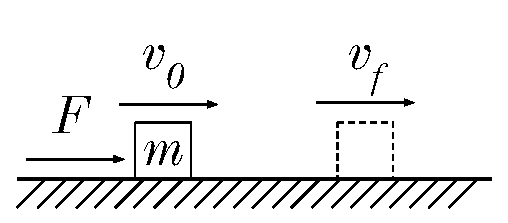
\includegraphics[width = \marginparwidth]{figures/scivola.pdf}
    \caption{Forza agente su una massa in moto}
\end{marginfigure}

Per rispondere al primo quesito, possiamo assumere un moto rettilineo
uniformemente accelerato durante l'intervallo $T$. Sappiamo che \[ a = \frac{F}{m} = \frac{dv}{dt} \]
Da cui possiamo esprimere la velocità in funzione del tempo (la velocità
iniziale la conosciamo già, ma assumiamo un tempo iniziale $t_0 = 0$):
\[ \frac{F}{m}dt = dv \to \int_{t_0}^{t}\frac{F}{m}dp = \int_{v_0}^{v}dw \to \frac{F}{m}\int_{0}^{t}dp = v - v_0 \to \frac{F}{m}t = v - v_0 \]
Dunque
\[ v(t) = v_0 + \frac{F}{m}t \]
Non ci manca che calcolare la velocità in corrispondenza di un $t_f = t_0 + \Delta t = 0 + T = T$:
\[ v(t_f) = v(T) = v_0 + \frac{F}{m}T \]

Nel secondo quesito, possiamo spezzare il problema in due parti: durante
l'azione della forza, la distanza percorsa ($s_a$) deve essere calcolata tenendo
conto del moto uniformemente accelerato, mentre nell'intervallo di tempo
successivo ($T_v$) il moto è semplicemente uniforme. Dalla seguente equazione,
possiamo ricavare $T_v$ ($T$ lo conosciamo già).
\[ s_w = s_a + s_v = s_a + v_fT_v = \int_{0}^{T}(v_0 + at)dp + v_fT_v = v_0T + \frac{1}{2}aT^2 + v_fT_v \]
Il tempo per percorrere $2\text{ km}$ è dunque:
\[ T_{2\text{ km}} = T + \frac{s_w - v_iT - \frac{F}{2m}T^2}{v_f} = T + \frac{s_w - v_iT - \frac{F}{2m}T^2}{v_i + \frac{F}{m}T} \]

\section{Lancio verso l'alto}
Si consideri la situazione mostrata in Figura \ref{lanciobasso}.
Durante la salita, l'oggetto rallenta a causa dell'accelerazione di gravità $g$.
Determiniamo la quota che l'oggetto raggiungerà.

\[ a = \frac{dv}{dt} \to dv = adt \to \int_{v_0}^{v}dw = \int_{t_0}^{t}adp \to v - v_0 = a\int_{t_0}^{t}dp \to v - v_0 = a(t - t_0) \]
Dunque
\[ v(t) = v_0 + a(t - t_0) = v_0 + at \]
Rallentando, si arriverà ad un istante $t_f$ nel quale l'oggetto avrà velocità
nulla:
\begin{marginfigure}
    \centering
    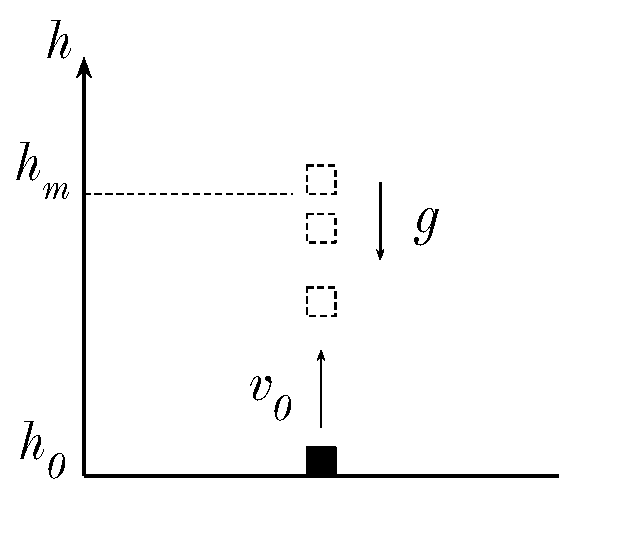
\includegraphics[width = \marginparwidth]{figures/greve.pdf}
    \caption{Lancio di un oggetto verso l'alto}
    \label{lanciobasso}
\end{marginfigure}
\[ v(t_f) = 0 \to v_0 + at_f = 0 \]
Non disponiamo tuttavia del tempo, ma possiamo avvalerci della legge oraria
che descrive la distanza percorsa:
\[ v(t) = \frac{dh}{dt} \to \int_{h_0}^{h}dk = \int_{t_0}^{t}v(t)dp \to h - h_0 = \int_{t_0}^{t}(v_0 + ap)dp \]
\[ h - h_0 = v_0\int_{t_0}^{t}dp + a\int_{t_0}^{t}pdp \to h - h_0 = v_0t + \frac12 at^2 \]
Da cui:
\[ h(t) = h_0 + v_0t + \frac12 at^2 = v_0t + \frac12 at^2 \]
Abbiamo quindi ottenuto la quota in funzione del tempo, che possiamo ricavare
dall'equazione $v_0 + at_f = 0 \to t_f = -\frac{v_0}{a}$.
\[ h(t_f) = v_0t_f + \frac12 at_{f}^2 =  -\frac{v_0^2}{a} + \frac{1}{2}a\frac{v_0^2}{a^2} = -\frac{v_0^2}{a} + \frac{v_0^2}{2a} = -\frac{v_0^2}{2a} \]
Sapendo che $a = -|g|$, la quota massima $h_m$ raggiunta è:
\[ h_m = \frac{v_0^2}{2|g|} \]

%%%%%%%%%%%%%%%%%%%%%%%%%%%%%%%%%%%%%%%%%%%%%%%%%%%%%%%%%%%%%%%%%

\subsection*{Spostamento}
\[ \Delta\overrightarrow{s} = \overrightarrow{s}_f - \overrightarrow{s}_i \]


\subsection{La terza legge}
\vspace{8pt}
\begin{tcolorbox}[colback = red!30, colframe = red!30!black, title = {Terza legge della dinamica (legge di azione e reazione)}]
La forza che un corpo $A$ esercita su un corpo $B$ è uguale e opposta alla forza
che

\[ \overrightarrow{F}_{A\to B} = -\overrightarrow{F}_{B\to A} \]
\end{tcolorbox}
\vspace{5pt}


\section{Statica}
\[ \sum_{i = 1}^{N}\overrightarrow{F}_i = m\overrightarrow{a} \]
La somma nel membro di sinistra è detta \textit{risultante} ($\overrightarrow{R}$).
In quiete, non c'è accelerazione:
\[ \overrightarrow{R} = \overrightarrow{0} \]
Se la velocità è costante, possiamo parlare di problemi di quiete? Yes.

\subsection*{Esercizio}
$\overrightarrow{P} + \overrightarrow{T} = \overrightarrow{0} \Rightarrow -mg + T = 0 \Rightarrow T = mg$.

\begin{marginfigure}
    \centering
    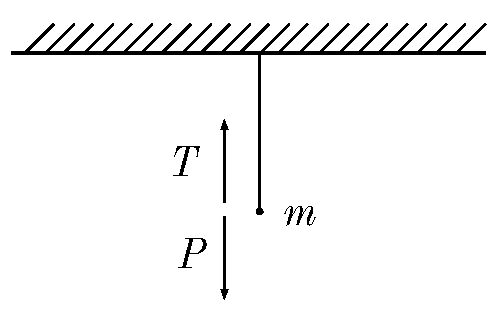
\includegraphics[width = \marginparwidth]{figures/statica.pdf}
    \caption{Massa appesa ad un filo}
    \label{filo}
\end{marginfigure}

\subsection*{Esercizio}
Come quello precedente ma con due corde che tengono $m$, inclinate di
tot gradi fissate al soffitto. Trovare la tensione su ciascun filo.




\section{Dinamica e moti armonici}
Tratteremo il moto armonico introducendo elementi di dinamica newtoniana,
studiando in particolare i cosiddetti \textit{oscillatori armonici}.
\vspace{8pt}
\begin{tcolorbox}[colback = yellow!30, colframe = yellow!30!black, title = {Oscillatore armonico}]
    Un oscillatore armonico è un oggetto su cui agisce una forza proporzionale,
    in modulo, allo spostamento dalla posizione di equilibrio e diretta in
    verso opposto rispetto a tale spostamento.
\end{tcolorbox}
\vspace{5pt}
Saranno due gli oscillatori armonici di nostro interesse: l'oscillatore a
molla e il pendolo semplice. Tuttavia, esistono numerosi esempi di oscillatori
armonici in natura, come uno snowboarder che compie evoluzioni in un half-pipe o
un atomo che vibra intorno al suo punto di equilibrio, il bilanciere di un
orologio (con le dovute approssimazioni).



\subsection{Le equazioni del moto armonico}
Riprendiamo le equazioni del moto armonico introdotto nel capitolo precedente.
Il cuore pulsante di tutte le leggi orarie del moto armonico è la funzione
periodica, seno o coseno. La scelta tra queste due dipende dal sistema di
riferimento scelto e dalle condizioni iniziali dell'oscillatore. Nel nostro
caso, scegliamo un oscillatore che parte dalla posizione di equilibrio
(e che come vedremo avrà velocità massima in questo punto), quindi utilizziamo
il seno per descrivere la sua posizione in funzione del tempo:
\[ x(t) = A\sin(\omega t) \]
È necessario fare alcune precisazioni: per \textit{posizione} non intendiamo
solo quella spaziale, ma anche, per esempio, quella angolare; inoltre,
l'equazione precedente non è sufficientemente generale, perché abbiamo
implicitamente supposto che l'istante temporale iniziale sia $t_0 = 0$. Per
questo, la legge oraria generale della posizione di un oscillatore armonico
è $x(t) = A\sin(\omega (t - t_0)) = A\sin(\omega t - \omega t_0)$ (è facile
verificare che effettivamente $x(t_0) = 0$, in accordo con la nostra scelta
del sistema di riferimento). In genere la legge si scrive in questo modo
\begin{align}
    x(t) = A\sin(\omega t + \phi)
\end{align}
Introduciamo alcune terminologie tecniche:
\begin{itemize}
    \item \textbf{Ampiezza} $A$: si tratta del massimo spostamento spaziale
    dell'osillatore a partire dal suo punto di equilibrio, in genere assunto
    come origine del sistema di riferimento adottato per la posizione. Nell'esempio del moto
    circolare, corrisponde al raggio della circonferenza. L'oscillatore si
    muove di fatto tra il massimo $A$ e il minimo $-A$.

    \item \textbf{Pulsazione} $\omega$: è un indice della ``rapidità''
    dell'oscillatore nel compiere i suoi cicli. Approfondiremo meglio
    l'interpretazione della pulsazione nei prossimi paragrafi.
    
    \item \textbf{Fase} $\phi = -\omega t_0$: intuitivamente, lo
    ``sfasamento'' dell'oscillatore. Incontriamo spesso oscillatori sfasati
    quando essi vengono messi in moto in istanti differenti. Per comodità,
    ometteremo spesso la fase, sottointendendo $t_0 = 0$.
\end{itemize}
Con qualche derivata della posizione, otteniamo velocità e accelerazione
dell'oscillatore in fuznione del tempo:
\[ v(t) = \frac{d}{dt}x(t) = \frac{d}{dt}(A\sin(\omega t + \phi)) = A\omega\cos(\omega t + \phi) \]
\[ a(t) = \frac{d}{dt}v(t) = \frac{d}{dt}(A\omega\cos(\omega t + \phi)) = -A\omega^2\sin(\omega t + \phi) \]
Ecco dunque le leggi orarie generali della velocità e dell'accelerazione di
un oscillatore armonico:
\begin{align}
    v(t) &= A\omega\cos(\omega t + \phi)\label{velarmonica}\\
    a(t) &= -A\omega^2\sin(\omega t + \phi)\label{accarmonica}
\end{align}
Concludiamo scrivendo la legge per eccellenza di un moto armonico, ovvero la
\textit{condizione sufficiente}. Sappiamo che l'accelerazione non è altro che
la derivata seconda della posizione rispetto al tempo:
\[ a = \frac{dv}{dt} = \frac{d^2x}{dt^2} \]
Ma dall'Equazione \ref{accarmonica} notiamo che
\[ a = -A\omega^2\sin(\omega t + \phi) = -\omega^2(A\sin(\omega t + \phi)) = -\omega^2x \]
Dunque
\begin{align}
    \frac{d^2x}{dt^2} + \omega^2x = 0
\end{align}
Abbiamo appena definito matematicamente l'oscillatore armonico: cinematicamente,
in un oscillatore l'accelerazione è proporzionale allo spostamento con costante
di proporzionalità negativa.

\subsubsection*{Interpretazione dell'ampiezza}
\subsubsection*{Interpretazione della fase}
\subsubsection{Interpretazione della pulsazione}
In tutte le equazioni dei moti armonici dominano le funzioni goniometriche.
Esse sono periodiche, ovvero esiste una quantità $T$ tale per cui $f(x + T) =
f(x)$ per ogni $x$ appartenente al dominio di $f$. In parole meno fredde,
dopo un certo \textit{periodo} la funzione si ripete, ciclicamente. Per seno
e coseno, il periodo corrisponde a $2\pi$ (infatti, vale per esempio $\sin(x+2\pi) =
\sin(x) \quad \forall x$).

Isoliamo la componente goniometrica delle equazioni armoniche, considerando
per esempio il seno e ignorando la fase $\phi$ (per il coseno il ragionamento
è analogo, mentre per $\phi$ possiamo risolvere il problema mediante trasformazioni).
Supponiamo di avere il periodo $T$, ovvero quel valore per cui la funzione ritorna
uguale a se stessa:
\[ \sin(\omega t) = \sin(\omega(t + T)) = \sin(\omega t + \omega T) \]
Sapendo che il periodo del seno è $2\pi$:
\[ \omega T = 2\pi \quad \therefore \quad \omega = \frac{2\pi}{T} \]
Possiamo dunque comprendere il significato della pulsazione $\omega$:
il suo valore è inversamente proporzionale al periodo $T$, ovvero la
pulsazione cresce al diminuire di $T$, e viceversa. Questo vuol dire
che $\omega$ fornisce un indice della ``rapidità'' con la quale le
oscillazioni di un moto armonico avvengono. Graficamente, $\omega$
comprime verso l'asse dell'ampiezza la funzione goniometrica quando il suo
valore cresce.

\subsection{L'oscillatore a molla}
Consideriamo un carrello di una rotaia a cuscino d'aria di massa $m$ attaccato
ad una molla di costante elastica $k$, indice della durezza della molla. Quando la molla si trova nella
posizione di equilibrio, cioè né estesa né compressa, il carrello rimane
fermo. Poniamo questa posizione come l'origine $x_o = 0$ di un asse delle
posizioni. Se il carrello viene spostato dall'equilibrio e portato a una
distanza $\overline{x}$ da tale posizione, la molla esercita una forza
elastica di \textit{richiamo} che, per la legge di Hooke, corrisponde a
\[ F = -k(x - x_o) = -kx \]
Il segno negativo indica appunto che si tratta di una forza di richiamo,
dunque opposta, nel suo verso, allo spostamento dalla posizione di equilibrio.
Possiamo applicare la seconda legge di newton:
\[ -kx = ma = m\frac{d}{dt}(v) = m\frac{d}{dt}\frac{d}{dt}(x) = m\frac{d^2x}{dt^2} \]
Da cui
\[ \frac{d^2x}{dt^2} + \frac{k}{m}x = 0 \]
È evidente che si tratta di un oscillatore armonico, perché l'accelerazione
è proporzionale allo spostamento, con costante di proporzionalità negativa.
Questa costante è $-\frac{k}{m} = -\omega^2$, da cui possiamo dedurre il
periodo dell'oscillatore a molla:
\begin{align}
    T = 2\pi\sqrt{\frac{m}{k}}\label{periodomolla}
\end{align}

\subsubsection*{Oscillatori verticali}
Anche una massa appesa ad una molla verticale può comportarsi come un
oscillatore armonico. L'unica differenza è la posizione di equilibrio,
nella quale il peso della massa eguaglia la forza di richiamo della
molla:
\[ mg = kx_0 \]
Indipendentemente dal sistema di riferimento utilizzato, l'equazione del
periodo non cambia. La forma delle equazioni armoniche rimane pressoché
invariata, ma è necessario fare attenzione ad eventuali traslazioni spaziali
derivanti dalla scelta del sistema di riferimento.

\subsubsection*{Misurare dinamicamente $k$ di molle per ammortizzatori}
Per misurare la costante elastica di una molla, è immediato tentare un approccio
statico, quindi allungando la molla, registrando la lunghezza di tale allungamento
e la forza di richiamo della molla in seguito alla deformazione. Esiste tuttavia
un metodo ancora più interessante che sfrutta le equazioni armoniche, in particolare
il periodo espresso nell'equazione \ref{periodomolla}.
\[ k = 4\pi^2\frac{m}{T^2} \]
Supponiamo di voler misurare la costante elastica dell'ammortizzatore di un'auto.
Con un po' di ingegno, deduciamo che se affrontiamo un dosso ad alta velocità
l'auto oscillerà verticalmente per qualche istante, per poi assestarsi. Possiamo
dunque stimare il tempo che l'auto impiega per compiere la primissima oscillazione,
che in realtà corrisponderà pressapoco alla metà del periodo di oscillazione.
Infine, conoscendo la massa dell'auto, è possibile utilizzare l'equazione precedente,
ma con una massa divisa per quattro, perché essa viene distribuita sulle quattro
ruote.

%$m = 1500\text{ kg}$ (massa di una ruota per quattro).
%\[ k = m_r\frac{4\pi^2}{T^2} = m\frac{\pi^2}{T^2} \simeq 1500\frac{10}{1\text{ s}}\text{ kg/s$^2$}\]
%$T \simeq 1\text{ s}$.


\subsection{Il pendolo}
Quello del pendolo semplice è un sistema fisico descrivibile mediante
il modello del moto armonico. Un pendolo semplice è formato da una massa
$m$ appesa ad un filo o un'asta (idealmente inestensibili e di massa
trascurabile) con una certa lunghezza $l$. Il punto di equilibrio stabile del pendolo si trova
esattamente al di sotto del punto di sospensione. Di fatto, la posizione
a riposo corrisponde a quella illustrata nel sistema della Figura
\ref{filo}, dove è stato appunto mostrato che la risultante delle
forze agenti sulla massa appesa è nulla.

Supponiamo di spostare la massa dalla sua posizione di equilibrio,
formando un angolo $\theta$ tra il filo e la verticale. Sappiamo che
la massa può oscillare lungo un arco di circonferenza. Fissiamo un
sistema di riferimento solidale alla massa, con un asse coincidente con
la retta passante per il filo e l'altro ad esso perpendicolare, dunque
tangente all'arco. Scomponiamo dunque il peso della massa lungo questi
assi (perpendicolare e tangenziale)  e applichiamo la seconda legge della
dinamica:
\[ ma_t = P_t = -mg\sin\theta \]
\[ ma_n = - P_n + T + F_c = 0 \]
Notare che nella seconda equazione è presente anche la forza centripeta
$F_c$ derivante dal moto circolare, oltre la tensione. Concentriamoci
sull'accelerazione tangenziale nella prima equazione. Ricordando che gli
angoli sono in relazione con la lunghezza degli archi $a$ secondo
l'equazione $a = l\theta$:
\[ a_t = \frac{dv_t}{dt} = \frac{d}{dt}\left(\frac{ld\theta}{dt}\right) = l\frac{d^2\theta}{dt^2} \]
Dunque, riprendendo la primissima equazione riguardo la componente
tangenziale del peso, semplificando la massa:
\[ l\frac{d^2\theta}{dt^2} + g\sin\theta = 0 \]
Per rendere più semplice la trattazione del sistema fisico, supporremo
per ipotesi che $\theta\ll 1$ (in radianti), dunque ciò che calcoleremo
in seguito varrà solamente per piccole oscillazioni del pendolo.
\marginpar{
    \footnotesize
    %\hspace*{-0.5cm}
    \begin{tabular}{c|c|c}
        Prima                      & $\varepsilon\to0$ & Dopo\\
        \hline
        $\sin\varepsilon$          &                   & $\varepsilon$\\
        $\tan\varepsilon$          &                   & $\varepsilon$\\
        $\cos\varepsilon$          &                   & $1 - \frac{\varepsilon^2}{2}$\\
        $e^\varepsilon$            &                   & $1 + \varepsilon$\\
        $(1 + \varepsilon)^\alpha$ &                   & $1 + \alpha\varepsilon$
    \end{tabular}
}
Ricordando le proprietà delle serie di Taylor, possiamo approssimare
il seno nella precedente equazione, dividere per la lunghezza $l$ del
pendolo ottenendo
\[ \frac{d^2\theta}{dt^2} + \frac{g}{l}\theta = 0 \]
Diventa dunque evidente il motivo della semplificazione: abbiamo ottenuto
una relazione nella quale l'accelerazione (angolare) dipende proporzionalmente
dallo spostamento (angolare) con costante di proporzionalità negativa.
In altre parole, si tratta della descrizione di un moto armonico semplice
nella forma $\frac{d^2x}{dt^2} + \omega^2 x = 0$, dalla quale si deduce
che $\omega^2 = \frac{g}{l}$. Ma sapendo che $\omega^2 = (\frac{2\pi}{T})^2$
abbiamo modo di determinare il periodo di oscillazione del pendolo:
\begin{align}
    T = 2\pi\sqrt{\frac{l}{g}}
    \label{periodopendolo}
\end{align}


\subsubsection*{Isocronia delle piccole oscillazioni}
Come già aveva concluso Galileo nel 1583, il periodo di oscillazione
del pendolo, ristretta ad angoli ridotti a partire dalla posizione
di equilibrio, non dipende dall'ampiezza, come altri moti armonici.
Questo fatto è dimostrato dall'equazione precedentemente ottenuta
(Equazione \ref{periodopendolo}). Ciò che rende un pendolo diverso
dall'altro è la lunghezza del filo e ``il pianeta su cui si trova'',
intendendo l'accelerazione gravitazionale $g$. Mantenendo invariati
questi parametri, possiamo fissare una qualsiasi massa $m$ e caricare
il pendolo a nostro piacere (sempre entro i limiti di angoli ridotti),
ma $T$ non cambierà.

Il fatto che l'oscillazione non dipenda dalla massa fissata trova una
motivazione analoga a quella di una massa in caduta libera, dove
l'accelerazione è sempre la stessa. Masse ridotte si muovono più
facilmente per la loro piccola inerzia, ma tuttavia su di esse agisce
una forza altrettanto ridotta; d'altra parte, masse maggiori sono
sottoposte a forze gravitazionali maggiori, ma sono anche più difficili
da spostare.
Per giustificare intuitivamente l'indipendenza dall'ampiezza, è
sufficiente pensare che una maggiore ``carica'' è compensata da un
tragitto maggiore (l'arco di circonferenza descritto durante
l'oscillazione).

Possiamo dunque concludere che queste compensazioni sono il motivo
delle indipendenze osservabili nell'equazione \ref{periodopendolo}.

\subsubsection*{Analisi approfondita del moto di un pendolo}
Alla luce delle equazioni sul moto armonico semplice, definiamo la
velocità \textit{angolare} di una massa di un pendolo semplice:
\[ \nu = \frac{d\theta}{dt} = A\omega\cos(\omega t + \phi) \]
Ricordiamo che l'ampiezza $A$ corrisponde all'angolo massimo spazzato
durante l'oscillazione, quindi si tratta di una grandezza adimensionale,
seppur col significato di radianti. Per quanto riguarda l'accelerazione
angolare:
\[ \alpha = \frac{d\nu}{dt} = -A\omega^2\sin(\omega t + \phi) \]
Descriviamo $a$, l'arco di circonferenza descritto durante il moto,
sapendo che la lunghezza del filo è $l$:
\[ a = l\theta = lA\sin(\omega t + \phi) \]
Per quanto riguarda velocità tangenziale e accelerazione tangenziale:
\[ v_t = \frac{da}{dt} = \frac{d}{dt}(l\theta) = l\frac{d\theta}{dt} = l\nu = lA\omega\cos(\omega t + \phi) \]
\[ a_t = \frac{dv}{dt} = -lA\omega^2\sin(\omega t + \phi) \]


\subsubsection*{Tensione del filo di un pendolo semplice in funzione del tempo}
All'inizio di questa sottosezione, abbiamo analizzato le forze in gioco
distinguendo le componenti tangenziali e perpendicolari alla circonferenza
descritta dal pendolo. È ora di analizzare la componente perpendicolare,
la quale permette al pendolo di non distruggersi durante l'oscillazione.
Infatti, la massa è mantenuta nella sua traiettoria per mezzo della tensione
del filo, che si contrappone alla componente perpendicolare del peso della
massa appesa più la forza centripeta derivante dal moto circolare in atto.
La relazione tra i moduli di queste forze è dunque la seguente:
\[T = P_\perp + F_c = mg\cos\theta + ma_c = mg\cos\theta + m\frac{v_t^2}{l} \]
Data la variazione di $\theta$ e di $v_t$ durante l'oscillazione, segue
che la tensione dipende dal tempo. Approssimiamo l'equazione supponendo
$\theta\ll1$, possiamo utilizziare
l'equazione della velocità tangenziale ottenuta precedentemente:
\[ T(t) = mg\cos\theta(t) + mlA^2\omega^2\cos^2(\omega t + \phi) \]
Per via delle approssimazioni, possiamo semplificare anche la funzione coseno
dipendente da $\theta$, rimanendo con il termine $mg(1-\frac{\theta^2}{2})$. Avendo la
descrizione armonica $\theta(t) = A\sin(\omega t + \phi)$ otteniamo la funzione
della tensione di un pendolo per piccole oscillazioni:
\begin{align}
    T(t) = mg\left(1 - \frac{(A\sin(\omega t + \phi))^2}{2}\right) + mlA^2\omega^2\cos^2(\omega t + \phi)
\end{align}

\section{Forze}
Il mondo che ci circonda è costituito da oggetti che esercitano delle azioni gli
uni sugli altri. Tali azioni impresse da agenti esterni su altri agenti sono
generalmente chiamate \textit{forze}, ma possono avere natura differente a seconda
del fenomeno fisico in esame. Ad esempio, le forze possono agire per contatto, come
la spinta delle ruote di un'auto sull'asfalto, o a distanza, come la forza di gravità.
Rimane tuttavia la caratteristica comune del loro \textit{effetto}, ovvero la capacità
di modificare il moto dei corpi in accordo con la seconda legge della dinamica.

\subsection{Peso}

\subsection{Forza elastica}

\subsection{Attrito}
Anche la più liscia delle superfici, se osservata a livello atomico, risulta
scabra. Per far scorrere due superfici l'una sull'altra, occorre superare la
resistenza dovuta agli urti fra i loro minuscoli avvallamenti e sporgenze. Questo
modello grossolano spiega intuitivamente l'origine della forza chiamata
\textit{attrito}. Esso dipende da molti fattori, come il materiale, la finitura
delle superfici, la presenza di lubrificanti, e pertanto non esiste una legge
fisica semplice ed universale che lo descriva. È tuttavia possibile derivare
alcune leggi empiriche in grado di calcolare le forze di attrito.

\subsubsection*{Attrito radente}
L'attrito radente si manifesta durante lo scivolamento tra due superfici (esiste
anche l'attrito volvente, che riguarda corpi estesi che rotolano e ruotano, ma non
è di nostro interesse dato lo studio del punto materiale). La forza di attrito
radente è proporzionale alla forza normale alla superficie ma è indipendente dalla
superficie di contatto fra le superfici ed è espressa dalla relazione
\[ \textbf{F}_A = \mu\mathbf{F}_\perp \]
dove $\mathbf{F}_\perp$ è la forza perpendicolare, o premente, alla superficie,
mentre $\mu$ è un coefficiente di attrito che dipende dai materiali degli oggetti
e altri fattori e spesso è compreso tra 0 e 1.

Le forze di attrito si suddividono a loro volta in attrito \textit{dinamico} e
\textit{statico}.

\subsubsection*{Attrito dinamico}
L'attrito dinamico si oppone allo scorrimento di un corpo su una superficie.

\subsubsection*{Attrito statico}
L'attrito statico si oppone al distacco di un corpo da una superficie. Esso tende
a impedire che un oggetto fermo su una superficie si distacchi da essa, cominciando
a scivolare. L'attrito statico è generalmente maggiore di quello dinamico, perché,
quando le supefici sono in contatto statico, i loro microscopici avvallamenti
(riprendiamo il modello introdotto per spiegare l'origine dell'attrito)
possono aderire maggiormente l'uno all'altro, determinando una maggiore
interazione tra superfici.

\subsubsection*{...}
$\overrightarrow{F_A} = \mu|\overrightarrow{N}|\hat{A}$. Grafico, zona statica
forza di attrito statica, regime dinamico forza di attrito dinamica.

Statica
\begin{align}
    \mathbf{F}_{A,S} = -\mathbf{F}_{\text{app}, T}\\
    |\mathbf{F}_{A,S} = |\mathbf{F}_{A,S}^\text{max}| = \mu_s|\mathbf{N}|
\end{align}
Dinamica
\begin{align}
    \mathbf{F}_{A,D} = -\mu_d|\mathbf{N}|\hat{v}
\end{align}